\documentclass[a4paper,12pt]{report}

\usepackage[utf8x]{inputenc}
\usepackage[T2A]{fontenc}
\usepackage[english, russian]{babel}

% Опционно, требует  apt-get install scalable-cyrfonts.*
% и удаления одной строчки в cyrtimes.sty
% Сточку не удалять!
% \usepackage{cyrtimes}

% Картнки и tikz
\usepackage{graphicx}
\usepackage{tikz}
\usetikzlibrary{snakes,arrows,shapes}


% Увы, поля придётся уменьшить из-за листингов.
\topmargin -1cm
\oddsidemargin -0.5cm
\evensidemargin -0.5cm
\textwidth 17cm
\textheight 24cm

\sloppy



% Оглавление в PDF
\usepackage[
bookmarks=true,
colorlinks=true, linkcolor=black, anchorcolor=black, citecolor=black, menucolor=black,filecolor=black, urlcolor=black,
unicode=true
]{hyperref}

% Для исходного кода в тексте
% \newcommand{\Code}[1]{\texttt{#1}}

% Некоторая русификация.
% \usepackage{misccorr} % Oh shi^W^W, оно не работает с report.
\usepackage{indentfirst}
\renewcommand{\labelitemi}{\normalfont\bfseries{--}}

% На дворе XXI век, но пакет listings всё ещё не пашет с русскими комментариями!

% Пакет listings для простой вставки исходников
% \usepackage{listings}
% Параметры оформления
% \lstset{
% showspaces=false,
% showtabs=false,
% frame=single,
% tabsize=4,
% basicstyle=\ttfamily,
% identifierstyle=\ttfamily,
% commentstyle=\itshape,
% stringstyle=\ttfamily,
% keywordstyle=\ttfamily,
% breaklines=true
% }
% Русский в комментариях.
% \lstset{escapebegin=\begin{cyr},escapeend=\end{cyr}}



% А это взято из файла, сгенерённого doxygen
\usepackage{calc}
\usepackage{array}
\newenvironment{Code}
{\footnotesize}
{\normalsize}
\newcommand{\doxyref}[3]{\textbf{#1} (\textnormal{#2}\,\pageref{#3})}
\newenvironment{DocInclude}
{\footnotesize}
{\normalsize}
\newenvironment{VerbInclude}
{\footnotesize}
{\normalsize}
\newenvironment{Image}
{\begin{figure}[H]}
{\end{figure}}
\newenvironment{ImageNoCaption}{}{}
\newenvironment{CompactList}
{\begin{list}{}{
  \setlength{\leftmargin}{0.5cm}
  \setlength{\itemsep}{0pt}
  \setlength{\parsep}{0pt}
  \setlength{\topsep}{0pt}
  \renewcommand{\makelabel}{\hfill}}}
{\end{list}}
\newenvironment{CompactItemize}
{
  \begin{itemize}
  \setlength{\itemsep}{-3pt}
  \setlength{\parsep}{0pt}
  \setlength{\topsep}{0pt}
  \setlength{\partopsep}{0pt}
}
{\end{itemize}}
\newcommand{\PBS}[1]{\let\temp=\\#1\let\\=\temp}
\newlength{\tmplength}
\newenvironment{TabularC}[1]
{
\setlength{\tmplength}
     {\linewidth/(#1)-\tabcolsep*2-\arrayrulewidth*(#1+1)/(#1)}
      \par\begin{tabular*}{\linewidth}
             {*{#1}{|>{\PBS\raggedright\hspace{0pt}}p{\the\tmplength}}|}
}
{\end{tabular*}\par}
\newcommand{\entrylabel}[1]{
   {\parbox[b]{\labelwidth-4pt}{\makebox[0pt][l]{\textbf{#1}}\vspace{1.5\baselineskip}}}}
\newenvironment{Desc}
{\begin{list}{}
  {
    \settowidth{\labelwidth}{40pt}
    \setlength{\leftmargin}{\labelwidth}
    \setlength{\parsep}{0pt}
    \setlength{\itemsep}{-4pt}
    \renewcommand{\makelabel}{\entrylabel}
  }
}
{\end{list}}
\newenvironment{Indent}
  {\begin{list}{}{\setlength{\leftmargin}{0.5cm}}
      \item[]\ignorespaces}
  {\unskip\end{list}}


\begin{document}

\tableofcontents
\setcounter{page}{3} % начать нумерацию с номера три
\addcontentsline{toc}{chapter}{Введение}
\chapter*{Введение}
\subsection{Цели и задачи}

Цель: 
    Разработать \textbf{SMTP-клиент} используя вызов select (или poll) и единственный рабочий процесс. Журналирование
    в отдельном процессе.

Задачи:
\begin{itemize}
    \item Проанализировать архитектурное решение
    \item Разработать подход для обработки исходящих соединений и отправки (пересылки) писем MTA-сервера из директории maildir
    \item Рассмотреть \textbf{SMTP}-протокол
    \item Реализовать программу для отправки писем по протоколу \textbf{SMTP}
    \item Реализовать метод журналирования в отдельном процессе\textbf{SMTP}
\end{itemize}

\chapter{Аналитический раздел}

\section*{Предметная область}
Согласно обозначенному протоколу в рамках данной работы, в системе устанавливаются отношения "отправитель - получатель", причем отправитель может отправить письмо нескольким получателям.
Основная единица данных, передаваемая по протоколу - письмо, которое включает в себя отправителя и получателя, причем получателей может быть несколько.
Также письмо содержит в себе единственное тело, которое может быть использовано как для последующей передачи, так и для хранения на сервере.
Таким образом, в рамках предметной области можно выделить 3 вида сущностей:
\begin{itemize}
    \item 1. Сервер
    \item 2. Клиент
    \item 3. Письмо
\end{itemize}
\section*{Клиент}
\subsection*{Преимущества и недостатки условия задачи}
Согласно условию задачи, в работе клиента предлагается исполльзовать однопроцессную асинхронную систему. Данная архитектура имеет следующие преимущества:
\begin{itemize}
    \item 1. Лучшая производительность по сравнению с простой многопроцессной (как и многопоточной) схемой за счёт оптимального использования ресурсов процесса в моменты его вынужденных "простоев" на какаом-либо соединении из-за неизбежных временных потерь ввиду "латентности" сетевой передачи данных.
    \item 2. Возможность не использовать потенциально подверженные сложноотлаживаемым ошибкам средства межпроцессного взаимодействия.
    \item 3. Любая прикладная задача представима в однопроцессной схеме работы (в отличие от параллельной, многопроцессной или многопоточной).
\end{itemize}
При этом данная архитектура имеет следующие недостатки:
\begin{itemize}
    \item 1. Сложность реализации. В отличие от многопроцессной или многопоточной схемы, асинхронная система подразумевает "пересечение" в одном потоке кода для выполнения сразу нескольких, логически независимых задач, что затрудняет их проектирование и отладку
    \item 2. Простая асинхронная обработка имеет свои границы масштабирования, за которыми необходимо объединять асинхронность с многопоточностью.
\end{itemize}
\chapter{Конструкторский раздел}

\section{Конечный автомат состояний клиента}

Конечный автомат состояний клиента представлен на Рис.~\ref{fig:client_fsm}

\begin{figure}
	\centering
	\includegraphics[width=\textwidth]{static/state_diagram_client.png}
	\caption{Состояния клиента}
	\label{fig:lient_fsm}
\end{figure}

\subsection{Синтаксис команд протокола}
Ниже приведен формат команд сообщений протокола в виде регулярных выражений
\begin{enumerate}
\item \textbf{EHLO}: {\it EHLO [w+]+\/}
\item \textbf{HELO}: {\it HЕLO [w+]+\/}
\item \textbf{MAIL}: {\it MAIL FROM <[\textbackslash w]+@[\textbackslash w]+\.[\textbackslash w]+>\/}
\item \textbf{RCPT}: {\it RCPT <[\textbackslash w]+@[\textbackslash w]+\.[\textbackslash w]+>\/}
\item \textbf{DATA}: {\it DATA\/}
\item \textbf{RSET}: {\it RSET\/}
\item \textbf{QUIT}: {\it QUIT\/}
\end{enumerate}

\subsection*{Представление данных}
Ниже приведена диаграмма представления данных в системе
\begin{figure}
\centering
\includegraphics[width=\textwidth]{static/physical_.png}
\caption{Физическая диаграмма сущностей}
\label{fig:phys_diagram}
\end{figure}


\subsection{Алгоритм обработки соединений}
\begin{verbatim}

 ПОКА (процесс_работает == 1)
        Проверить директорию почты maildir на наличие необработанных сообщений
        ЕСЛИ сообщения есть, создать новый клиентский_сокет
        КОНЕЦ ЕСЛИ

        ОБНУЛИТЬ список_сокетов
        ДЛЯ каждого клиентского_сокета:
            добавить клиентский_сокет в список_сокетов,
            ЕСЛИ список_сокетов НЕ пуст:
                применить SELECT (или POLL) для получения списка дескрипторов на чтение (ДЧ), запись (ДЗ)
                ДЛЯ каждого дескриптора в ДЧ:
                    выбрать клиентский_сокет из списка_сокетов
                    запустить для него обработчик_состояний_FSM_для чтения_из_сокета
                КОНЕЦ ДЛЯ

                ДЛЯ каждого дескриптора в ДЗ:
                    выбрать клиентский_сокет из списка_сокетов
                    запустить для него обработчик_состояний_FSM для записи_в_сокет
                КОНЕЦ ДЛЯ
            КОНЕЦ ЕСЛИ
        КОНЕЦ ДЛЯ
 КОНЕЦ ПОКА

\end{verbatim}

\chapter{Технологический раздел}

\section{Сборка программы}

Сборка программы описана в файле \textit{Makefile} системы сборки \textit{make}. Рис.~\ref{fig:make}. Изображение с конечным автоматом генерируется срествами библиотеки transitions.

\begin{figure}
\centering
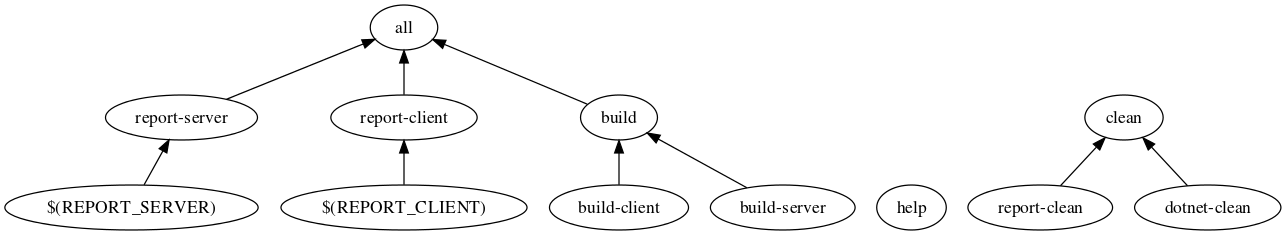
\includegraphics[width=\textwidth]{include/make.png}
\caption{Сборка программы}
\label{fig:make}
\end{figure}

\section{Графы вызова функций}

Поскольку функций много, графы вызовов разбиты на два рисунка. На рис.~\ref{fig:cflow01} показаны основные функции, на рис.~\ref{fig:cflow02}~-- функции обработки команд. 

\begin{figure}
\centering
\includegraphics[width=\textwidth]{static/smtp-course-work14_.png}
\caption{Граф вызовов}
\label{fig:cflow01}
\end{figure}

\vspace{100mm}

\section{Тестирование}

Ниже приведён отчет о модульном тестировании.

\begin{verbatim}

Testing started at 10:44 ...
/home/sbn/PycharmProjects/smtp-course-work/venv/bin/python /home/sbn/Downloads/pycharm-community-2019.3.1/plugins/python-ce/helpers/pycharm/_jb_pytest_runner.py --target test_sockets.py::test_send_simple_message_socket
Launching pytest with arguments test_sockets.py::test_send_simple_message_socket in /home/sbn/PycharmProjects/smtp-course-work/client/tests

============================= test session starts ==============================
platform linux -- Python 3.8.0, pytest-5.3.2, py-1.8.1, pluggy-0.13.1 -- /home/sbn/PycharmProjects/smtp-course-work/venv/bin/python
cachedir: .pytest_cache
rootdir: /home/sbn/PycharmProjects/smtp-course-work/client/tests
plugins: cov-2.8.1
collecting ... collected 2 items

test_sockets.py::test_send_simple_message_socket PASSED                      [100%]
test_reg_exp_s.py::test_ALL_patterns_CLIENT PASSED                      [100%]

============================== 2 passed in 10.60s==============================

\end{verbatim}
\addcontentsline{toc}{chapter}{Выводы}
\chapter*{Выводы}

В рамках предложенной работы нами был реализован SMTP-клиент в соответствии со стандартами RFC. В ходе работы реализованы следующие задачи: \\
\begin{enumerate}
	\item Проанализировали архитектурное решение
    \item Разработан подход для обработки исходящих соединений и отправки исходящих писем MTA-сервера из директории maildir
    \item Рассмотрен \textbf{SMTP}-протокол
    \item Реализована программа для отправки писем по протоколу \textbf{SMTP}
    \item Рассмотрена работа с неблокирующими сокетами и их взаимодействие
    \item Реализован метод журналирования в отдельном процессе\textbf{SMTP}
    \item Разработана система, работающая в многозадачном режиме (основной процесс, процесс журналирования и т.д.)
    \item Произведено ознакомление с утилитами автоматической сборки и тестирования
\end{enumerate}
В ходе работы получены следующие навыки: \\
\begin{enumerate}
\item проектирования реализации сетевого протокола по имеющейся спецификации;
\item реализации сетевых приложений на языке программирования;
\item реализации сетевой службы без создания нити на каждое соединение;
\item автоматизированного системного тестирования ПО сетевой службы;
\item групповой работы с использованием системы контроля версий;
\end{enumerate}


\end{document}
